\documentclass[10pt, bachelor,subf,href,colorlinks=true
%,fixint=false
%,times
]{disser}

\usepackage[
  a4paper, mag=1000, includefoot,
  left=2.5cm, right=1.5cm, top=2cm, bottom=2cm, headsep=1cm, footskip=1cm
]{geometry}
\usepackage{mathtext}
\usepackage[T2A]{fontenc}
\usepackage[utf8]{inputenc}
%\usepackage{ucs}
\usepackage[english,russian]{babel}
\usepackage{graphicx}
\usepackage{cmap}
%\usepackage{subfig}
%\usepackage{tikz}
%\usepackage{float}
%\usepackage{caption}
\usepackage[font=small]{subcaption}
%AMS TEX значки и пр.
\usepackage{amssymb, amsthm, amsmath}
\usepackage[noend]{algorithmic}
%\usepackage{array}
\usepackage{tabularx}
\usepackage{multicol, multirow}
\usepackage{ragged2e}
\ifpdf\usepackage{epstopdf}\fi

% Номера страниц сверху и по центру
%\def\headfont{\small}
%\pagestyle{headcenter}
%\chapterpagestyle{empty}

% Использовать полужирное начертание для векторов
\let\vec=\mathbf

% Включать подсекции в оглавление
\setcounter{tocdepth}{2}

\graphicspath{{pics/}}

\numberwithin{equation}{section}
\begin{document}
\newcommand{\hmax}{\ensuremath{h^{max}}}
\newcommand{\hmin}{\ensuremath{h^{min}}}

\newcommand{\hini}[1]{h^{(i)}_{#1}}
\newcommand{\hfin}[1]{h^{(f)}_{#1}}

\newcommand{\Tin}{\ensuremath{T^{in}}}
\newcommand{\Tout}{\ensuremath{T^{out}}}
\newcommand{\Tres}{\ensuremath{T^{res}}}
\newcommand{\tin}{\ensuremath{t^{in}}}
\newcommand{\tout}{\ensuremath{t^{out}}}
\newcommand{\tres}{\ensuremath{t^{res}}}
\newcommand{\PER}{\ensuremath{q}}
\newcommand{\Iin}{\ensuremath{I^{in}}}
\newcommand{\Idis}{\ensuremath{I^{dis}}}
\newcommand{\Iout}{\ensuremath{I^{out}}}

\newcommand{\Qmax}{\ensuremath{Q^{max}}}

\renewcommand{\le}{\leqslant}
\renewcommand{\ge}{\geqslant}

\newcommand{\pin}{\ensuremath{p^{in}}}
\newcommand{\Pin}{\ensuremath{P^{in}}}
\newcommand{\pout}{\ensuremath{p^{out}}}
\newcommand{\Pout}{\ensuremath{P^{out}}}



\institution{Московский физико-технический институт \\ (государственный университет) \\ Факультет радиотехники и кибернетики \\ Кафедра проблем передачи и обработки информации}

% Имя лица, допускающего к защите (зав. кафедрой)
\apname{академик РАН А.П. Кулешов}

\title{Выпускная квалификационная работа\\БАКАЛАВРА}

\topic{Передача мультимедийных данных в сетях Wi-Fi Mesh с помощью механизма детерминированного доступа}

% Автор
\author       {Иванов А.С.} % ФИО
\group        {011} % Группа
\coursenum    {010900} % Номер направления
\course       {Прикладные математика и физика}
%\masterprognum{010674} % Номер магистерской программы
%\masterprog   {Телекоммуникационные сети и системы}

% Научный руководитель
\sa      {Хоров Е.М.}
\sastatus{к.~т.~н.}

% Рецензент
%\rev      {Якимов М.Ю.}
%\revstatus{к.~т.~н.}

% Консультант
%\conspec{вопросам\\охраны труда}
%\con{ФИО консультанта}
%\constatus{к.~т.~н., доц.}

% Город и год
\city{Москва}
\date{\number\year}

\maketitle
\newpage

\tableofcontents

\intro

\textbf{Актуальность задачи.} С ростом популярности сервисов реального времени растут как объемы генерируемых ими мультимедийных данных, так и требования пользователей к качеству обслуживания таких данных, т.е. QoS-требования (Quality of Service).  QoS-требования данных реального времени включают в себя как минимальную пропускную способность, так и ограничения на задержку передачи и долю потерянных пакетов PLR (Packet Loss Ratio). Выполнение QoS-требований при передаче мультимедийных данных с минимальными затратами канальных ресурсов является одной из наиболее актуальных задач в области беспроводных коммуникаций.

%Постоянно растущие требования пользователей к качеству обслуживания (QoS-требования) отражают изменения в структуре трафика в интернете. В частности, мультимедийный трафик (который производится такими приложениями, как VoIP, HD TV, видеоконференции и т.д.) занимает все больше и больше сетевых ресурсов. Поскольку ранние стандарты Wi-Fi поддерживали только  best effort transmissions, новые решения от Wi-Fi сообщества должны учитывать нужды пользователей.

%The constantly increasing users requirements for Quality of Service (QoS) reflect changes in the overall structure of the traffic in the Internet. In particular, multimedia traffic (generated by applications like VoIP, videoconferencing, High Definition TV, etc.) is occupying more and more network resources. QoS requirements of multimedia traffic include not only a minimal bandwidth but also a bounded delay and packet loss ratio. Since the early Wi-Fi standards were designed only for best effort transmissions, new solutions from the Wi-Fi community are requested to keep pace with the users needs. 

%As a response the IEEE 802.11 Working Group for WLAN Standards has produced the IEEE 802.11e amendment aimed to provide QoS support. 
%Particularly, the amendment introduced 
%The special attention paid to channel access methods is connected to a fact that in wireless networks the ability to provide QoS to a considerable degree depends on available channel access methods. Actually, in the last decade the IEEE 802.11 Working Group has made a number of steps in this direction. 

В Wi-Fi сетях возможность выполнения QoS-требований зависит от используемых механизмов доступа к каналу.   При использовании механизмов \textit{детерминированного} доступа станции передают в заранее зарезервированных ими интервалах времени. С одной стороны, передачи в зарезервированных интервалах защищены от коллизий, поскольку станции не ведут передачу в чужих интервалах. С другой стороны, изменение зарезервированных интервалов занимает существенное время, затрачиваемое на согласование новых параметров зарезервированных интервалов с соседними станциями. Такие задержки могут быть особенно критичны в случае передачи мультимедийных потоков реального времени, кратковременные всплески интенсивности которых вынуждают либо изменять параметры зарезервированных интервалов, либо резервировать канальные ресурсы с избытком.

При использовании механизмов \textit{случайного} доступа станции выбирают случайные моменты времени для передачи данных. Это обеспечивает б\'{о}льшую гибкость по сравнению с детерминированным доступом, поскольку при их использовании для передачи данных можно попытаться получить доступ к каналу после того, как он оказался свободным в течение некоторого промежутка времени, а не ждать ближайшего зарезервированного интервала. По этой причине механизмы случайного доступа эффективны в случаях резкого увеличения интенсивности передаваемых потоков. В то же время таким механизмам свойственны частые коллизии (особенно в плотных сетях) и случайные задержки при попытках получить доступ к каналу. В результате механизмы случайного доступа не могут гарантировать выполнение QoS-требований при передаче данных реального времени. 

%In wireless networks, the ability to provide QoS to a considerable degree depends on available channel access methods. That is why the first Wi-Fi amendment aimed for QoS support --- IEEE 802.11e~\cite{802.11e} --- has paid a special attention to this issue by defining two QoS-oriented channel access mechanisms: Enhanced Distributed Channel Access (EDCA) and Hybrid coordination function Controlled Channel Access (HCCA). The former is a \textit{random} (contention-based) channel access mechanism and provides prioritized QoS. The latter is an example of \textit{deterministic} channel access and provides parameterized QoS by means of contention-free polling.

%+ deterministic channel access schedule and other staff One of the key lying in the basis of reliable data transmission is deterministic channel access. Generally speaking, a deterministic channel access methods allow a station to preliminarily reserve a set of

%Механизмы детерминированного доступа, основанные на предварительном резервировании канала, обеспечивают б\'{о}льшую надежность передачи по сравнению с механизмами случайного доступа, поскольку последние существенно страдают от множественных коллизий. В то же время детерминированный доступ обладает меньшей гибкостью, нежели случайный доступ, так как требует времени на изменение зарезервированных интервалов. Последнее особенно критично в случае передачи мультимедийных потоков.

%С точки зрения передачи мультимедийных потоков, механизмы случайного доступа обладают б\'{о}льшей гибкостью, так как при их использовании для передачи данных не обязательно ждать ближайшего зарезервированного интервала, а можно попытаться получить доступ к каналу после того, как он оказался свободным в течение некоторого промежутка времени. Поэтому механизмы случайного доступа эффективны для поглощения всплесков интенсивности передаваемых потоков, хоть и имеют меньшую надежность передачи по сравнению с механизмами детерминированного доступа.   

Механизм детерминированного доступа может быть улучшен за счет гибкости случайного доступа,  если использовать эти два вида доступа совместно в составе некоторого механизма \textit{комбинированного} доступа: основная часть потока может быть передана внутри зарезервированных интервалов, в то время как для поглощения всплесков интенсивности передаваемого потока дополнительно задействуется случайный доступ. Комбинированный доступ обещает значительные выгоды как с точки зрения возможности выполнения QoS-требований (за счет передачи внутри защищенных зарезервированных интервалов), так и с точки зрения объема используемого канального времени (не нужно резервировать время с расчётом на наибольшую возможную интенсивность входного потока, а только для передачи его постоянной составляющей). Основной вопрос заключается в том, как именно нужно использовать механизмы комбинированного доступа при передаче данных реального времени.

%Гибкость случайного доступа и надежность детерминированного доступа могут быть достигнуты одновременно, если использовать эти два вида доступа совместно в составе некоторого механизма \textit{комбинированного} доступа: основная часть потока может быть передана внутри зарезервированных интервалов, в то время как для поглощения всплесков интенсивности передаваемого потока дополнительно задействуется случайный доступ. Комбинированный доступ обещает значительные выгоды как с точки зрения возможности выполнения QoS-требований (за счет передачи внутри защищенных зарезервированных интервалов), так и с точки зрения объема используемого канального времени (не нужно резервировать время с рассчетом на наибольшую возможную интенсивность входного потока, а только для передачи его постоянной составляющей). Основной вопрос заключается в том, как именно нужно использовать механизмы комбинированного доступа при передаче данных реального времени.


%Высокая плотность сети подразумевает наличие большого числа точек доступа (AP) в одной области , that is, in Overlapping Basic Service Sets (OBSSs). Недостаток доступных для передачи частот заставляет соседние точки доступа передавать на одной и той же частоте. В случае использования EDCA в плотной сети эффективность этого механизма резко падает по причине существенной интерференции между станциями и частых коллизий. HCCA в состоянии лишь немного улучшить ситуацию, поскольку передача точки доступа, использующей HCCA, защищена только от пересечения с передачами станций (STA), ассоциированных с этой точкой доступа, но не с передачами других точек доступа. По этим причинам ни EDCA ни HCCA не могут предоставлять приемлемый уровень качества обслуживания в подобных ситуациях потому что они не предназначены для использования в сетях с высокой плотностью. Чтобы улучшить работу OBSS, дополнение IEEE 802.11aa, разработанное для робасной передачи аудио и видеопотоков добавило в HCCA the HCCA Negotiation procedure. Эта процедура позволяет точкам доступа резервировать интервалы времени, в течение которых точка доступа опрашивает свои станции, в то время как соседние точки доступа (вместе со своими станциями) не ведут передачу. Это и достигается за счет HCCA Negotiation, что подразумевает распространение точками доступа информации о зарезервированных интервалах. Данный подход существенно улучшает надежность передачи за счет дополнительных затрат. Для того чтобы уменьшить эти затраты, интервалы времени резервируются не по одному, а в рамках целой последовательности: точка доступа может резервировать \textit{последовательность периодически повторяющихся интервалов времени равной длительности}, что мы в дальнейшем будем называть \textit{периодическим резервированием}. Основная идея заключается в том, что всё резервирование может быть описано с помощью всего лишь трех величин: \textit{период} зерезервированных интервалов, их \textit{продолжительность} и \textit{момент начала первого интервала} (см рис.~\ref{fig:periodic_reservation}). 

%The further evolution of wireless technologies has leaded to the emergence of new scenarios of Wi-Fi application implying high network density. The high density results in coexistence of a high number of access points (APs) in the same area, that is, in Overlapping Basic Service Sets (OBSSs). The lack of the available spectrum makes neighboring APs to operate at the same frequency channel. In case of OBSSs EDCA performance degrades dramatically due to severe interference and frequent collisions. HCCA is able only to slightly relieve the situation, since HCCA when used by some AP protects data transmissions only from stations (STAs) associated with this AP, but not from other STAs. Thus, both EDCA and HCCA fail to provide acceptable QoS in such scenarios since neither of them is meant for high density. To improve the performance of OBSSs, the IEEE 802.11aa amendment, which is developed for robust audio and video streaming, has extended HCCA with the HCCA Negotiation procedure. This procedure allows an AP to reserve time intervals during which the AP polls its STAs while the neighboring APs (along with their STAs) keep silent. The latter is what is achieved through HCCA Negotiation which makes APs to disseminate the information about the reserved time intervals. It increases transmission reliability though at the cost of the additional overhead. In order to reduce the overhead, time intervals are reserved not individually but in sequences: an AP can reserve \textit{a sequence of periodic time intervals of equal duration} which we further refer to as a \textit{(periodic) reservation}. The key idea is that the whole reservation can be described only by three parameters: the \textit{period} of the reserved time intervals, their \textit{duration} and the \textit{beginning of the first interval} (see Fig.~\ref{fig:periodic_reservation}). 

 %В дополнении IEEE 802.11ah, которое нацелено на адаптацю Wi-Fi к использованию в интернете вещей~\cite{khorov2014survey}, резервирования используются для того, чтобы сократить конкуренцию за доступ к каналу между тысячами сенсоров. Также обсуждается возможность включить периодические резервирования в дополнение IEEE 802.11ax (High Efficiency WLAN), которое представляет собой новое поколение Wi-Fi.

%The advantages of periodic reservations have made them current among recent Wi-Fi amendments. The IEEE 802.11s amendment designed for Wi-Fi Mesh introduces Mesh coordination function Controlled Channel Access (MCCA). MCCA allows any STA in a Wi-Fi Mesh network to set up a periodic reservation in order to protect its transmissions from interference with neighboring STAs. In the IEEE 802.11ah amendment, which aims to adapt Wi-Fi to the Internet of Things scenarios~\cite{khorov2014survey}, reservations are used to reduce the contention between thousands of sensors. Periodic reservations are also discussed to be included into the IEEE 802.11ax (High Efficiency WLAN) amendment, which represents a new generation of Wi-Fi. %is constitues subject of the IEEE 802.11 Working Group.

%It is worth to mention that deterministic access methods based on periodic reservations differ from ordinary polling-based access methods, e.g. PCF (Point Coordination Function) and HCCA (from IEEE 802.11e), in the need for establishing reservations \textit{in advance} so that all neighboring STAs can be informed about them. That is why changes in the parameters (period and duration) of an established reservation require quite long time spent on a) parameters negotiation with neighboring STAs for preventing overlapping of reservations and b) sending information about new parameters. Consequently, such changes become highly undesirable especially when serving traffic with QoS requirements. 
 
\textbf{Задачей данной работы} является анализ использования механизма комбинированного доступа для передачи мультимедийных данных реального времени и разработка метода выбора таких его параметров, при которых выполнены QoS-требования к передаче потока, а потребление канальных ресурсов минимально. Для решения данной задачи в работе разработана математическая модель передачи мультимедийного потока с использованием  механизма комбинированного доступа. Данная модель позволяет сравнить механизм комбинированного доступа с механизмом детерминированного доступа в плане потребления канальных ресурсов с необходимыми для выполнения QoS-требованиями к передаче потока. При построении математической модели были использованы такие \textbf{методы исследования}, как теория вероятностей и комбинаторный анализ.    

%Хотя периодические резервирования являются эффективным подходом при обслуживании потока данных постоянной интенсивности (CBR), они показывают худшие результаты при обслуживании потока переменной интенсивности (VBR)~\cite{turletti2003fhcf, grilo2002performance, cowling2004detailed, cecchetti2011real}. Это происходит из-за невозможности поменять параметры резервирований быстро, чтобы подстроиться под вариации VBR-трафика, в то время как неправильный выбор таких параметров приводит к нарушениям налагаемых QoS-требований. Единственная возможность преодолеть эту проблему средствами детерминированного доступа это зарезервировать доступ к каналу в избытке, чтобы справиться с пиковой нагрузкой VBR-потока. Очевидно, что такой подход приводит к излишнему потреблению канальных ресурсов и потому оказывается неэффективным. 

%Though being efficient when serving Constant Bit Rate flows (CBR), periodic reservations demonstrate poor performance when serving VBR flows~\cite{turletti2003fhcf, grilo2002performance, cowling2004detailed, cecchetti2011real}. It happens because of the inability to change the reservation parameters quickly to match time-varying nature of VBR flows, while a wrong choice of a polling or reservation period leads to violation of QoS requirements. The only way to overcome this problem by means of the deterministic access is to reserve a redundant amount of the channel time to account for the highest rate of an incoming VBR flow. Obviously, such an approach could lead to excessive channel time wastes and turns out to be inefficient. 

%As shown in \cite{turletti2003fhcf, grilo2002performance, cowling2004detailed, cecchetti2011real} through comprehensive analytical and simulation modeling (in the context of periodic HCCA-based polling), periodic reservations and polling perform well when transmitting CBR (Constant Bit Rate) flows. However those studies also demonstrate poor performance of deterministic access for VBR (Variable Bit Rate) flows. It is due to the inability to change the reservation parameters quickly to match time-varying nature of VBR flows, while a wrong choice of a polling or reservation period leads to violation of QoS requirements. The only way to overcome this problem by means of the deterministic access is to reserve a redundant amount of channel time to account for the highest rate of an incoming VBR flow. Obviously, such an approach could lead to excessive channel time wastes and turns out to be inefficient. 

%From the perspective of VBR flows, random access methods (like EDCA) promise higher flexibility. Indeed, they do not need to wait for the nearest reserved interval to transmit data and can start a contention for the channel after it remains idle for a specified duration. Thus, while not being efficient for transmitting a QoS-sensitive flows due to the backoff-induced delays and frequent collisions, the random access is able to handle variations of a VBR flow arrival rate. 

%The flexibility of random access methods and the reliability of deterministic ones could be combined together if these methods are jointly used: the most of a VBR flow data can be transmitted in reserved intervals protected from interference whereas the bursts of the flow can be handled with a random access method. A \textit{joint method} promises high gains in terms of both channel resource consumption and QoS provisioning. The main question is how it should work. In particular, how reserved time intervals should be placed and when a STA should use a random channel access method. The first attempt to answer this question is made by the IEEE 802.11e amendment which describes an additional access function called HCCA-EDCA Mixed Mode (HEMM). However, HEMM is not described well and only few studies \cite{kuan2007utilization, lai2009adaptation, Ng2012, ruscelli2012enhancement} consider its usage for QoS provisioning.

%The flexibility of random access methods and the reliability of deterministic ones could be combined together if these methods are jointly used.  Indeed, while the most in that case bursts of incoming VBR traffic can be absorbed with contention-based random access. If random access is not used, the only way to handle data bursts is to reserve redundant amount of channel time accounting for the highest incoming traffic intensity. That is why high gains are expected from the joint usage of two functions in terms of both channel resource consumption and QoS provisioning. The only question is how to choose parameters of such a usage. For example, how reserved time intervals should be places and when a STA should use random channel access. The first attempt to answer this question is made by the IEEE 802.11e amendment which describes an additional access function called HCCA-EDCA Mixed Mode (HEMM). The main problem with HEMM is that it is not described well and only few studies [9-11] consider its usage for QoS provisioning.
%\textbf{TODO Analyze results}
%Finally, the problem of joint usage still remains open.

%In this paper, we propose a joint channel access method and apply it to transmission of a VBR flow. We built a mathematical model of this process which can be used to find parameters of the joint method which guarantees meeting the QoS requirements of the flow with the minimal channel resource consumption. Moreover, we demonstrate the gain of the joint access by comparing it with the usage of the only access method.

\textbf{Научная новизна} данной работы заключается в том, что в ней разработана наиболее точная математическая модель процесса передачи мультимедийного потока с использованием механизма комбинированного доступа с учетом QoS-требований и возможных ошибок при передаче пакетов. 

\textbf{Положение, выносимое на защиту.} В данной работе была разработана математическая модель процесса передачи мультимедийного потока с использованием механизма комбинированного доступа. Разработанная модель позволяет найти такие параметры комбинированного доступа, при которых выполнены QoS-требования передаваемого потока, а потребление канальных ресурсов минимально. На основе полученной модели был разработан алгоритм динамического выбора параметров резервирования в случае передачи видеопотока в режиме реального времени.

%\textbf{Данная работа построена следующим образом.} В разделе~\ref{sec:methods} приводится краткое описание рассматриваемых в работе механизмов доступа, обзор существующих работ и  формальная постановка задачи. Раздел~\ref{sec:math_model} посвящен построению математической модели рассматриваемого процесса передачи. В разделе~\ref{sec:numerical} разработанная модель применяется для выбора параметров передачи, демонстрируется выгода от использования предложенного механизма доступа по сравнению с использованием механизма детерминированного доступа. Наконец, итоги работы приводятся в заключении.

%The rest of the paper is organized as follows. In Section~\ref{sec:related_papers}, we briefly review the existing studies on a joint usage of access methods. In Section~\ref{sec:problem_statement}, the problem of the paper is accurately formulated. Section~\ref{sec:math_model} is devoted to a mathematical model of the considered system. In Section~\ref{sec:numerical_results}, we show how the model can be applied to select appropriate transmission parameters and demonstrate benefits of the proposed joint channel access. Finally, Section~\ref{sec:conclusion} concludes the paper.
\section{Постановка задачи}
\label{sec:problem_title}

\subsection{Методы доступа к среде}
\label{sec:methods}

%Постоянно растущие требования пользователей к качеству обслуживания (QoS-требования) отражают изменения в структуре трафика в интернете. В частности, мультимедийный трафик (который производится такими приложениями, как VoIP, HD TV, видеоконференции и т.д.) занимает все больше и больше сетевых ресурсов. Поскольку ранние стандарты Wi-Fi поддерживали только  best effort transmissions, новые решения от Wi-Fi сообщества должны учитывать нужды пользователей.

%The constantly increasing users requirements for Quality of Service (QoS) reflect changes in the overall structure of the traffic in the Internet. In particular, multimedia traffic (generated by applications like VoIP, videoconferencing, High Definition TV, etc.) is occupying more and more network resources. QoS requirements of multimedia traffic include not only a minimal bandwidth but also a bounded delay and packet loss ratio. Since the early Wi-Fi standards were designed only for best effort transmissions, new solutions from the Wi-Fi community are requested to keep pace with the users needs. 

%As a response the IEEE 802.11 Working Group for WLAN Standards has produced the IEEE 802.11e amendment aimed to provide QoS support. 
%Particularly, the amendment introduced 
%The special attention paid to channel access methods is connected to a fact that in wireless networks the ability to provide QoS to a considerable degree depends on available channel access methods. Actually, in the last decade the IEEE 802.11 Working Group has made a number of steps in this direction. 

Дополнение IEEE 802.11e~\cite{802.11e} к стандарту Wi-Fi, направленное на внедрение поддержки QoS-требований, определило два новых механизма доступа: EDCA (Enhanced Distributed Channel Access) и HCCA (Hybrid coordination function Controlled Channel Access). Первый из них является механизмом приоритезированного случайного доступа к каналу, а второй -- механизмом детерминированного доступа.

С ростом плотности Wi-Fi-сетей HCCA и EDCA оказались не способны обеспечить надежную передачу данных, так как не обладают возможностями по работе в условиях жесткой интерференции. В частности, в случае большого числа точек доступа, работающих в одной области пространства, многие точки доступа выбирают один и тот же частотный канал. В результате EDCA страдает от множественных коллизий и эффекта скрытых станций. Ситуация с HCCA лишь немногим лучше за счет того, что HCCA исключает интерференцию со станциями своей сети. Поэтому возникает необходимость в разработке новых механизмов доступа, рассчитаных на работу в плотных сетях Wi-Fi.

Например, дополнение IEEE 802.11aa определяет механизм HCCA TXOP Negotiation, который позволяет точке доступа зарезервировать последовательность периодических интервалов времени, в течение которых она опрашивает свои станции, а соседние точки доступа (вместе со своими станциями) хранят молчание.  Данный подход существенно уменьшает интерференцию с соседними сетями, повышая надежность передачи. Стоит отметить, что интервалы времени резервируются не по одному, а целыми последовательностями: точка доступа резервирует \textit{последовательность периодических интервалов времени равной длительности}, в дальнейшем называемую \textit{периодическим резервированием}. Благодаря периодичности, все резервирование может быть описано с помощью всего лишь трех величин: \textit{периода} зерезервированных интервалов, их \textit{длительности} и \textit{момента начала первого интервала} (рис.~\ref{fig:periodic_reservation}).

\begin{figure}[h]
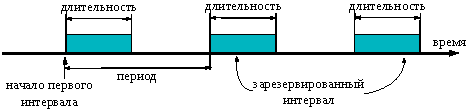
\includegraphics[width=\linewidth]{ReservedIntervals.pdf}
\caption{\label{fig:periodic_reservation} Периодическое резервирование}
\end{figure} 

%In wireless networks, the ability to provide QoS to a considerable degree depends on available channel access methods. That is why the first Wi-Fi amendment aimed for QoS support --- IEEE 802.11e~\cite{802.11e} --- has paid a special attention to this issue by defining two QoS-oriented channel access mechanisms: Enhanced Distributed Channel Access (EDCA) and Hybrid coordination function Controlled Channel Access (HCCA). The former is a \textit{random} (contention-based) channel access mechanism and provides prioritized QoS. The latter is an example of \textit{deterministic} channel access and provides parameterized QoS by means of contention-free polling.

%+ deterministic channel access schedule and other staff One of the key lying in the basis of reliable data transmission is deterministic channel access. Generally speaking, a deterministic channel access methods allow a station to preliminarily reserve a set of

%Дальнейшее развитие беспроводных технологий привело к появлению новых возможностей использования Wi-Fi в условиях высокой плотности сети. Высокая плотность сети подразумевает наличие большого числа точек доступа (AP) в одной области , that is, in Overlapping Basic Service Sets (OBSSs). Недостаток доступных для передачи частот заставляет соседние точки доступа передавать на одной и той же частоте. В случае использования EDCA в плотной сети эффективность этого механизма резко падает по причине существенной интерференции между станциями и частых коллизий. HCCA в состоянии лишь немного улучшить ситуацию, поскольку передача точки доступа, использующей HCCA, защищена только от пересечения с передачами станций (STA), ассоциированных с этой точкой доступа, но не с передачами других точек доступа. По этим причинам ни EDCA ни HCCA не могут предоставлять приемлемый уровень качества обслуживания в подобных ситуациях потому что они не предназначены для использования в сетях с высокой плотностью. Чтобы улучшить работу OBSS, дополнение IEEE 802.11aa, разработанное для робасной передачи аудио и видеопотоков добавило в HCCA the HCCA Negotiation procedure. Эта процедура позволяет точкам доступа резервировать интервалы времени, в течение которых точка доступа опрашивает свои станции, в то время как соседние точки доступа (вместе со своими станциями) не ведут передачу. Это и достигается за счет HCCA Negotiation, что подразумевает распространение точками доступа информации о зарезервированных интервалах. Данный подход существенно улучшает надежность передачи за счет дополнительных затрат. Для того чтобы уменьшить эти затраты, интервалы времени резервируются не по одному, а в рамках целой последовательности: точка доступа может резервировать \textit{последовательность периодически повторяющихся интервалов времени равной длительности}, что мы в дальнейшем будем называть \textit{периодическим резервированием}. Основная идея заключается в том, что всё резервирование может быть описано с помощью всего лишь трех величин: \textit{период} зерезервированных интервалов, их \textit{продолжительность} и \textit{момент начала первого интервала} (см рис.~\ref{fig:periodic_reservation}). 

%The further evolution of wireless technologies has leaded to the emergence of new scenarios of Wi-Fi application implying high network density. The high density results in coexistence of a high number of access points (APs) in the same area, that is, in Overlapping Basic Service Sets (OBSSs). The lack of the available spectrum makes neighboring APs to operate at the same frequency channel. In case of OBSSs EDCA performance degrades dramatically due to severe interference and frequent collisions. HCCA is able only to slightly relieve the situation, since HCCA when used by some AP protects data transmissions only from stations (STAs) associated with this AP, but not from other STAs. Thus, both EDCA and HCCA fail to provide acceptable QoS in such scenarios since neither of them is meant for high density. To improve the performance of OBSSs, the IEEE 802.11aa amendment, which is developed for robust audio and video streaming, has extended HCCA with the HCCA Negotiation procedure. This procedure allows an AP to reserve time intervals during which the AP polls its STAs while the neighboring APs (along with their STAs) keep silent. The latter is what is achieved through HCCA Negotiation which makes APs to disseminate the information about the reserved time intervals. It increases transmission reliability though at the cost of the additional overhead. In order to reduce the overhead, time intervals are reserved not individually but in sequences: an AP can reserve \textit{a sequence of periodic time intervals of equal duration} which we further refer to as a \textit{(periodic) reservation}. The key idea is that the whole reservation can be described only by three parameters: the \textit{period} of the reserved time intervals, their \textit{duration} and the \textit{beginning of the first interval} (see Fig.~\ref{fig:periodic_reservation}). 

Кроме дополнения IEEE 802.11aa периодические резервирования также присутствуют и в дополнении IEEE 802.11s (описывающим сети Wi-Fi Mesh). Это дополнение определяет механизм детерминированного доступа MCCA (Mesh coordination function Controlled Channel Access). MCCA позволяет любой станции в сети Wi-Fi Mesh установить периодическое резервирование, чтобы защитить собственные передачи от интерференции с соседними станциями. %В дополнении IEEE 802.11ah, которое нацелено на адаптацю Wi-Fi к использованию в интернете вещей~\cite{khorov2014survey}, резервирования используются для того, чтобы сократить конкуренцию за доступ к каналу между тысячами сенсоров. Также обсуждается возможность включить периодические резервирования в дополнение IEEE 802.11ax (High Efficiency WLAN), которое представляет собой новое поколение Wi-Fi.

%The advantages of periodic reservations have made them current among recent Wi-Fi amendments. The IEEE 802.11s amendment designed for Wi-Fi Mesh introduces Mesh coordination function Controlled Channel Access (MCCA). MCCA allows any STA in a Wi-Fi Mesh network to set up a periodic reservation in order to protect its transmissions from interference with neighboring STAs. In the IEEE 802.11ah amendment, which aims to adapt Wi-Fi to the Internet of Things scenarios~\cite{khorov2014survey}, reservations are used to reduce the contention between thousands of sensors. Periodic reservations are also discussed to be included into the IEEE 802.11ax (High Efficiency WLAN) amendment, which represents a new generation of Wi-Fi. %is constitues subject of the IEEE 802.11 Working Group.

%Стоит отметить, что описанные выше механизмы детерминированного доступа (MCCA, HCCA TXOP Negotiation) резервируют канал \textit{заранее}, чтобы все соседние станции знали о них. При этом внесение изменений в параметры установленных резервирований занимает продолжительное время, которое затрачивается на согласование новых параметров с параметрами резервирований соседних станций, чтобы избежать пересечения резервирований. Поэтому такие изменения являются крайне нежелательными, особенно при передаче данных с жесткими QoS-требованиями.

%It is worth to mention that deterministic access methods based on periodic reservations differ from ordinary polling-based access methods, e.g. PCF (Point Coordination Function) and HCCA (from IEEE 802.11e), in the need for establishing reservations \textit{in advance} so that all neighboring STAs can be informed about them. That is why changes in the parameters (period and duration) of an established reservation require quite long time spent on a) parameters negotiation with neighboring STAs for preventing overlapping of reservations and b) sending information about new parameters. Consequently, such changes become highly undesirable especially when serving traffic with QoS requirements. 

%Механизмы детерминированного доступа, основанные на предварительном резервировании канала, обеспечивают б\'{о}льшую надежность передачи по сравнению с механизмами случайного доступа. В то же время детерминированный доступ обладает меньшей гибкостью, нежели случайный доступ, так как требует времени на внесение изменений в установленные резервирования. Последнее особенно критично в случае передачи мультимедийных потоков реального времени, всплески интенсивности которых вынуждают резервировать значительно больше ресурсов с расчетом на максимальную интенсивность потока. Очевидно, что такой подход приводит к излишнему потреблению канальных ресурсов и потому неэффективен. 


%Хотя периодические резервирования являются эффективным подходом при обслуживании потока данных постоянной интенсивности (CBR), они показывают худшие результаты при обслуживании потока переменной интенсивности (VBR)~\cite{turletti2003fhcf, grilo2002performance, cowling2004detailed, cecchetti2011real}. Это происходит из-за невозможности поменять параметры резервирований быстро, чтобы подстроиться под вариации VBR-трафика, в то время как неправильный выбор таких параметров приводит к нарушениям налагаемых QoS-требований. Единственная возможность преодолеть эту проблему средствами детерминированного доступа это зарезервировать доступ к каналу в избытке, чтобы справиться с пиковой нагрузкой VBR-потока. Очевидно, что такой подход приводит к излишнему потреблению канальных ресурсов и потому оказывается неэффективным. 

%Though being efficient when serving Constant Bit Rate flows (CBR), periodic reservations demonstrate poor performance when serving VBR flows~\cite{turletti2003fhcf, grilo2002performance, cowling2004detailed, cecchetti2011real}. It happens because of the inability to change the reservation parameters quickly to match time-varying nature of VBR flows, while a wrong choice of a polling or reservation period leads to violation of QoS requirements. The only way to overcome this problem by means of the deterministic access is to reserve a redundant amount of the channel time to account for the highest rate of an incoming VBR flow. Obviously, such an approach could lead to excessive channel time wastes and turns out to be inefficient. 

%As shown in \cite{turletti2003fhcf, grilo2002performance, cowling2004detailed, cecchetti2011real} through comprehensive analytical and simulation modeling (in the context of periodic HCCA-based polling), periodic reservations and polling perform well when transmitting CBR (Constant Bit Rate) flows. However those studies also demonstrate poor performance of deterministic access for VBR (Variable Bit Rate) flows. It is due to the inability to change the reservation parameters quickly to match time-varying nature of VBR flows, while a wrong choice of a polling or reservation period leads to violation of QoS requirements. The only way to overcome this problem by means of the deterministic access is to reserve a redundant amount of channel time to account for the highest rate of an incoming VBR flow. Obviously, such an approach could lead to excessive channel time wastes and turns out to be inefficient. 

%С точки зрения передачи мультимедийных потоков, механизмы случайного доступа, такие как EDCA, обладают б\'{о}льшей гибкостью, так как при их использовании для передачи данных не обязательно ждать ближайшего зарезервированного интервала, а можно попытаться получить доступ к каналу после того, как он оказался свободным в течение некоторого промежутка времени. Поэтому механизмы случайного доступа эффективны для поглощения всплесков интенсивности передаваемых потоков, хоть и имеют меньшую надежность передачи по сравнению с механизмами детерминированного доступа.

%From the perspective of VBR flows, random access methods (like EDCA) promise higher flexibility. Indeed, they do not need to wait for the nearest reserved interval to transmit data and can start a contention for the channel after it remains idle for a specified duration. Thus, while not being efficient for transmitting a QoS-sensitive flows due to the backoff-induced delays and frequent collisions, the random access is able to handle variations of a VBR flow arrival rate. 

При использовании механизма комбинированного доступа для передачи мультимедийных данных реального времени с учетом QoS-требований, необходимо ответить на вопрос о том, как должны быть размещены зарезервированные интервалы времени, и когда станция должна использовать механизм случайного доступа. Первая попытка ответить на этот вопрос была сделана в дополнении  IEEE 802.11e, которое описывает механизм доступа, называемый HEMM (HCCA-EDCA Mixed Mode). Однако, HEMM описан недостаточно хорошо и только несколько работ  \cite{kuan2007utilization, lai2009adaptation, Ng2012, ruscelli2012enhancement} рассматривают использование этого механизма для передачи данных с QoS-требованиями.

%The flexibility of random access methods and the reliability of deterministic ones could be combined together if these methods are jointly used: the most of a VBR flow data can be transmitted in reserved intervals protected from interference whereas the bursts of the flow can be handled with a random access method. A \textit{joint method} promises high gains in terms of both channel resource consumption and QoS provisioning. The main question is how it should work. In particular, how reserved time intervals should be placed and when a STA should use a random channel access method. The first attempt to answer this question is made by the IEEE 802.11e amendment which describes an additional access function called HCCA-EDCA Mixed Mode (HEMM). However, HEMM is not described well and only few studies \cite{kuan2007utilization, lai2009adaptation, Ng2012, ruscelli2012enhancement} consider its usage for QoS provisioning.

%The flexibility of random access methods and the reliability of deterministic ones could be combined together if these methods are jointly used.  Indeed, while the most in that case bursts of incoming VBR traffic can be absorbed with contention-based random access. If random access is not used, the only way to handle data bursts is to reserve redundant amount of channel time accounting for the highest incoming traffic intensity. That is why high gains are expected from the joint usage of two functions in terms of both channel resource consumption and QoS provisioning. The only question is how to choose parameters of such a usage. For example, how reserved time intervals should be places and when a STA should use random channel access. The first attempt to answer this question is made by the IEEE 802.11e amendment which describes an additional access function called HCCA-EDCA Mixed Mode (HEMM). The main problem with HEMM is that it is not described well and only few studies [9-11] consider its usage for QoS provisioning.
%\textbf{TODO Analyze results}
%Finally, the problem of joint usage still remains open.

%In this paper, we propose a joint channel access method and apply it to transmission of a VBR flow. We built a mathematical model of this process which can be used to find parameters of the joint method which guarantees meeting the QoS requirements of the flow with the minimal channel resource consumption. Moreover, we demonstrate the gain of the joint access by comparing it with the usage of the only access method.

%The rest of the paper is organized as follows. In Section~\ref{sec:related_papers}, we briefly review the existing studies on a joint usage of access methods. In Section~\ref{sec:problem_statement}, the problem of the paper is accurately formulated. Section~\ref{sec:math_model} is devoted to a mathematical model of the considered system. In Section~\ref{sec:numerical_results}, we show how the model can be applied to select appropriate transmission parameters and demonstrate benefits of the proposed joint channel access. Finally, Section~\ref{sec:conclusion} concludes the paper.
\subsection{Обзор существующих работ}
\label{sec:related_papers}

Часть работ, рассматривающих совместное использование случайного и детерминированного доступа, посвящены тому, как именно распределять ресурсы между этими механизмами. Например,~\cite{siris2006resource} показывает, как разделить ресурсы между EDCA и HCCA для достижения максимальной пропускной способности в сетях IEEE 802.11e. Сосуществование двух механизмов доступа также рассмотрено в~\cite{Krasilov2013} в рамках использования EDCA и MCCA в сетях Wi-Fi Mesh. \cite{Krasilov2013}~показывает, как количество зарезервированного времени влияет на пропускную способность EDCA. Однако в данных работах не рассмотрены ни совместное использование двух механизмов доступа для передачи одного потока данных, ни вопрос выполнения QoS-требований. 

%A number of papers devoted to both random and deterministic access study how to share resources between these methods.
%For example,~\cite{siris2006resource} gives recommendation on how to share resources between EDCA and HCCA to achieve the maximum overall throughput in IEEE 802.11e networks. The coexistence of the methods is also studied in~\cite{Krasilov2013} in terms of EDCA and MCCA in Wi-Fi Mesh networks. \cite{Krasilov2013}~shows how the amount of the reserved channel time influences the throughput of EDCA. But no QoS provisioning or joint usage is considered in both~\cite{siris2006resource} and~\cite{Krasilov2013}.

Что касается комбинированного использования двух механизмов доступа, то на эту тему существует всего лишь несколько работ, и все они в основном рассматривают HEMM. К примеру, \cite{kuan2007utilization} рассматривает ситуацию, в которой несколько станций передают в режиме насыщения, используя как EDCA, так и HCCA. Показано, что чем больше данных передается с помощью HCCA, тем больше доля времени, потраченного на успешные передачи. \cite{Ng2012}~предлагает использовать марковский процесс принятия решений для координирования HCCA и EDCA в сетях  IEEE 802.11e. Однако \cite{Ng2012}~не учитывает QoS-требования и ставит задачей лишь увеличение доли времени, потраченного на успешные передачи. Кроме того, ни  \cite{kuan2007utilization} ни \cite{Ng2012} не изучают применение HEMM для передачи потока с QoS-требованиями.

%As for the joint access, only a few studies exist so far and they mainly consider HCCA-EDCA Mixed Mode (HEMM). For example, \cite{kuan2007utilization} considers a scenario where a set of STAs transmit saturated traffic using both EDCA and HCCA. It is shown that the more data is transmitted with HCCA the higher is the channel utilization, that is, the percentage of time spend for successful transmissions. \cite{Ng2012}~proposes to use a Markov decision process for coordinating HCCA and EDCA in IEEE 802.11e networks. However, \cite{Ng2012}~considers no QoS requirements and aims only to improve the channel utilization. 
%In this paper, we propose a joint access method. But neither \cite{kuan2007utilization} nor \cite{Ng2012} study the ability of HEMM to transmit QoS-sensitive data. 

Влияние HEMM на выполнение QoS-требований рассмотрено в~\cite{ruscelli2012enhancement}, где представлены описание и анализ EDCA, HCCA и HEMM. \cite{ruscelli2012enhancement} предлагает улучшенный алгоритм управления доступом, который применяется для HEMM и может быть использован для улучшения показателей практически любого HCCA планировщика, что подтверждено имитационным моделированием. При этом не было разработано математической модели, которая могла бы быть использована для настройки параметров комбинированного доступа для поддержки QoS-требований.  

%The influence of HEMM on QoS provisioning is studied in~\cite{ruscelli2012enhancement} where a good description/analysis of EDCA, HCCA as well as HEMM can be found. \cite{ruscelli2012enhancement} proposes an enhanced admission control algorithm which accounts for HEMM and can be used to improve performance of almost any HCCA scheduler as shown by simulation. However, no analytical model, which can be used to study how joint access is efficient for supporting QoS, has been developed so far. Realizing this gap, we try to fill it in the current paper.

\subsection{Формальная постановка задачи}
\label{sec:problem_statement}

Рассмотрим передачу мультимедийного потока реального времени между двумя соседними станциями.  Считается, что пакеты потока поступают в очередь пачками частично известного размера, а именно первые $n$ пачек поступают в очередь с известным размером, после чего размер пачки принимает значение $i$ при учёте распределения размеров пачек уже известного на данный момент видеопотока $B(t)_{det}$ с вероятностью $p_i$, $i \in \{1, \ldots, M\}$), где $M$ --- максимально возможный размер пачки. Период поступления пачек --- $\Tin$, что соответствтует передаче видеопотока с использованием протокола RTP. Далее такой поток будем называть периодическим, неординарным и коррелированным, то есть размер каждой следующей пачки в каждый момент времени зависит от известного на данный момент распределения размеров пачек. QoS-требования представлены а) ограничением на время доставки пакета $\DQoS$ и б) ограничением на долю потерянных пакетов $\PLRQoS$. Если время нахождения пакета в очереди превышает $\DQoS$, то пакет отбрасывается, внося вклад в PLR.

Отправитель передает поток с использованием механизма комбинированного доступа, который работает следующим образом.
Отправитель устанавливает периодическое резервирование  с периодом $\Tres \leq \Tin$ и длительностью каждого зарезервированного интервала, рассчитанной ровно на одну попытку передачи пакета.
Отправитель всегда передает первый пакет из очереди.
%Для каждого пакета отправитель поддерживает счетчик передач: пакет может быть передан не более чем $\nretries$ раз.
%Спустя $\nretries$ попыток передачи пакет покидает очередь.
Также пакет покидает очередь, если был успешно передан, либо если его время нахождения в очереди превысило $\DQoS$.
Отправитель передает пакеты, используя либо детерминированный доступ (передавая пакеты в зарезервированных интервалах), либо случайный доступ. 
Передача с использованием случайного доступа ведется в промежутках между зарезервированными интервалами, т.е. в интервалах случайного доступа.
При этом пакет передается с использованием случайного доступа только тогда, когда он устаревает к началу следующего зарезерезвированного интервала.
Такой подход позволяет бороться со всплесками интенсивности и при 
этом позволяет сохранять минимальное потребление канальных ресурсов.
В интервале случайного доступа можно совершить ограниченное количество попыток передач.
Время между двумя попытками передач в интервале случайного доступа считается  экспоненциально-распределенной случайной величиной с параметром $\lambda$. 

Вероятность неуспешной передачи пакета внутри зарезервированного интервала равна $\qdet$, а в течение интервала случайного доступа --- $\qran \geq \qdet$. 

При таком использовании механизма комбинированного доступа основной вопрос состоит в том, как выбрать параметр $\Tres$, чтобы выполнить QoS-требования, используя при этом как можно меньше канального времени. Для ответа на этот вопрос была разработана математическая модель рассматриваемого процесса передачи. Эта модель позволяет найти PLR как функцию от $\Tres$ и по зависимости $PLR(\Tres)$ найти искомый параметр.

Также был разработан алгоритм нахождения максимального значения $\Tres$, при котором выполняются QoS-требования, в динамическом режиме, учитывающий состояние очереди в моменты принятия решения, а также распределение размеров пришедших к этому моменту пачек.

%В течении зарезервированного интервала передача пакета происходит неудачно с вероятностью $\perm$. Если для передачи используется метод случайного доступа (пакет передается за пределами зарезервированного интервала), то передача происходит неудачно с вероятностью $\pere$. 

%Мы также предполагаем, что в какой бы момент до следующего зарезервированного интервала пакет ни устарел, времени на совершение всех необходимых передач с использованием метода случайного доступа будет достаточно. 

%Наконец, \textit{пакет отбрасывается, если он не был передан успешно, только если его счетчик количества попыток передач достигает значения $\nretries$}.         







\chapter{Математическая модель одиночной передачи пакетов}
\label{chapter:model_noBlockAck}

В работе было рассмотрено несколько математических моделей...

\section{Аналитическая модель передачи}
\label{analyticalModel1}
\subsection{Цепь Маркова}

Представим $\Tin/\Tres$ в виде несократимой дроби $\tin/\tres$, где $\tin, \tres\in\mathbb{N}$. Назовем слотом интервал времени длины $$\tau = \frac{\Tin}{\tin} \equiv \frac{\Tres}{\tres}.$$ Разобьем непрерывную временную шкалу на слоты таким образом, чтобы начало каждого MCCAOP совпадало с началом некоторого слота -- см.~рис~\ref{fig:time}.

Процесс передачи пакетов с помощью механизма MCCA может быть описан цепью Маркова с дискретным временем, единица которого равна периоду резервирований.

\begin{figure}[t]
\centering{\includegraphics[width=0.7\linewidth]{pics/time1}}
	\caption{\label{fig:time}Слотированное время}
\end{figure}


В каждый момент времени $t$ состояние системы будем описывать парой целых чисел $(h(t), m(t), n(t))$. Если $h(t) \geqslant 0$, то очередь не пуста, и $h(t)$ равно числу полных слотов, которые головная (самая старшая) пачка пакетов провела в очереди, $m(t)$ равно числу пакетов в этой пачке, а $n(t)$ равно начальному числу пакетов в головной пачке. Если $h(t) < 0$, то очередь пуста, и $|h(t)|$ равно времени до прибытия новой пачки пакетов, выраженному в слотах и округленному вниз; при этом $m=0$. Таким образом, состояние системы в каждый моменты времени $t$ характеризуется текущим числом пакетов в головной пачке, начальным числом пакетов  в головной пачке и временем, в течение которого пакеты этой пачки ожидают передачи. Используемые обозначения состояния системы позволяют определить количество пачек пакетов в очереди:  $\lfloor h(t)/\tin \rfloor + 1$, но не позволяют определить длины всех пачек, кроме головной. После того, как все пакеты головной пачки были переданы или отброшены, определяется число пакетов в пачке, ставшей головной.
  
Минимальное значение $h(t)$ равно $\tres-\tin$. Оно достигается в момент времени $t$, если пачка из одного пакета пребывает в пустую очередь непосредственно перед моментом $t - 1$, и единственный пакет пачки успешно передается с первой попытки.   

Теперь найдем максимальное возможное значение $h(t)$. Для этого обозначим через $\xi$ время между поступлением пачки пакетов в очередь и началом следующего слота, $0 \leqslant \xi < \tau$. В силу того, что время $\Tin$ равно целому числу $\tin$ слотов, значение величины $\xi$ одинаково для всех пачек. Таким образом, к моменту времени $t$ время ожидания в очереди пакетов головной пачки равно $h(t) \cdot \tau + \xi$. Чтобы эта пачка не была отброшена в момент $t$, ее время ожидания не должно превышать значения $D$. Следовательно, $h(t) \leqslant d = \lfloor \frac{D-\xi}{\tau} \rfloor$. 

Благодаря тому, что числа $\tin$ и $\tres$ взаимно просты, цепь Маркова обладает свойством эргодичности. Таким образом, может быть найдено стационарное распределение вероятностей цепи Маркова. 

Выясним, в какие состояния и с какой вероятностью может перейти система из состояния $(h, m, n)$ за один шаг. Для этого отдельно рассмотрим несколько случаев.

\paragraph{1.} Пусть $h(t) < 0$, т.~е. в момент времени $t$ очередь пуста. 

\begin{itemize}
\item Если $h + \tres \ge 0$, то к моменту времени $t + 1$ в очередь поступит очередная пачка пакетов. Размер пачки является случайной величиной, подчиняющейся распределению условных вероятностей $p_{ji}$, где $j$ и $i$ --- размеры соседних пачек,  поэтому с вероятностью $p_{ni}$ система окажется в состоянии $(h + \tres, i, i)$. 

\item Если же $h + \tres < 0$, то к моменту времени $t + 1$ в очередь  не поступит ни одного пакета, т.~е. в этом случае система с вероятностью $1$ перейдет в состояние $(h + \tres, 0, n)$. 
\end{itemize}


\paragraph{2.} Пусть $h(t) \ge 0$ и $m(t) = 1$, т.~е. в головной пачке находится единственный пакет.

С вероятностью $1 - q$ происходит успешная передача пакета.

\begin{itemize}
\item Если при этом $h - \tin + \tres < 0$, то к моменту времени $t + 1$ на станцию не поступит ни одной пачки данных и система окажется в состоянии $(h - \tin + \tres, 0, n)$ с указанной выше вероятностью $1 - q$.
\item Если же $h - \tin + \tres \geqslant 0$, то в момент времени $t + 1$ очередь будет не пуста, и состояние системы будет определяться числом пакетов $i$ в головной пачке. Поскольку вероятность успешной попытки передачи пакета равна  $1 - q$, а пачка имеет размер $i$ с вероятностью $p_{ni}$, то система перейдет в состояние $(h - \tin + \tres, i, i)$, $i \in \{1, \dots, M\}$, с вероятностью $(1 - q)p_{ni}$.
\end{itemize} 

С вероятностью $q$ попытка передачи пакета оказывается неудачной. 

\begin{itemize}
\item Если $h + \tres > d$, то к моменту времени $t + 1$ время ожидания данного пакета  превысит допустимое значение $D$, и этот пакет будет отброшен. Cистема c вероятностью $qp_{ni}$ перейдет в одно из состояний $(h - \tin + \tres, i, i)$, $i \in \{1, \dots, M\}$.
\item Если $h + \tres \le d$, то к моменту времени $t + 1$ пакет не устареет, и будет предпринята следующая попытка передачи. Следовательно, система перейдет в состояние $(h + \tres, 1, n)$ с вероятностью $q$, а в состояние $(h + \tres, 0, n)$ с вероятностью $1 - q$.
\end{itemize} 

\paragraph{3.} Наконец, рассмотрим случай, когда $h(t) \geqslant 0$, $m(t) > 1$. 

С вероятностью $1 - q$ попытка передачи пакета была успешной. В этом случае в обслуживаемой пачке остается $m - 1$ пакет. 

\begin{itemize}
\item Если $h + \tres > d$, то к моменту времени $t + 1$ время ожидания этих пакетов превысит допустимое значение $D$, и все пакеты пачки будут отброшены. Система с вероятностью $(1-q)p_{ni}$ перейдет в одно из состояний $(h - \tin + \tres, i, i)$, $i \in \{1, \dots, M\}$. 
\item Если $h + \tres \le d$, то система с вероятностью $1-q$ перейдет в состояние $(h + \tres, m - 1, n)$.
\end{itemize} 

Аналогично, в случае, когда попытка передачи не была успешной, система перейдет в состояние $(h - \tin + \tres, i, i)$ при  $h + \tres > d$ с вероятностью $q p_{ni}$ и в $(h + \tres, m, n)$ --- при $h + \tres \le d$ с вероятностью $q$.

\paragraph{Подводя итог,} получаем, что при выполнении соответствующих условий система  переходит из состояния $(h, m)$ в одно из следующих состояний:

\begin{tabular}{l l l l}
1)	&$(h + \tres, 0, n)$, 			&$\gamma = 1$, 	&при $m = 0$, $h < -\tres$; \\
2)  &$(h + \tres, i, i)$, 			&$\gamma = p_{ni}$, &при $m = 0$, $-\tres \leqslant h < 0$; \\
3)  &$(h + \tres - \tin, i, i)$, 	&$\gamma = (1 - q)p_{ni}$, &при $m = 1$, $\tin - \tres \leqslant h \leqslant d$; \\
4)  &$(h + \tres - \tin, 0, n)$, 	&$\gamma = 1 - q$, &при $m = 1$, $0 \leqslant h < \tin - \tres$; \\
5)  &$(h + \tres - \tin, i, i)$, 	&$\gamma = q p_{ni}$, &при $m = 1$, $d - \tres < h \leqslant d$; \\
6)  &$(h + \tres, m, n)$, 			&$\gamma = q$, &при $m > 0$, $0 \leqslant h \leqslant d - \tres$; \\
7)  &$(h + \tres - \tin, i, i)$,	&$\gamma = p_{ni}$, &при $m > 1$, $d - \tres < h \leqslant d$; \\
8)  &$(h + \tres, m - 1, n)$, &$\gamma = 1 - q$, &при $m > 1$, $0 \leqslant h \leqslant d - \tres$;
\end{tabular} \newline
где $i\in\{1,\dots,M\}$ и $\gamma$ --- вероятность перехода. 

Уделим особое внимание переходу под номером~$7$. Он может осуществиться двумя способами. 

Первый способ заключается в том, что сначала с вероятностью $1 - q$ происходит успешная передача пакета, а потом с вероятностью $p_i$ переход в состояние $(h + \tres - \tin, i, i)$. Таким образом, вероятность перехода первым способом равна $(1 - q) p_{ni}$.

Второй способ заключается в том, что сначала с вероятностью $q$ возникает ошибка при передаче пакета, а затем с вероятностью $p_{ni}$ переход в состояние $(h + \tres - \tin, i, i)$. Получаем, что  вероятность перехода вторым способом равна $q p_{ni}$, а суммарная вероятность перехода $7$ равна $p_{ni}$. 

Однако между этими двумя способами реализации перехода есть существенное различие: при~первом способе отбрасывается $m - 1$ пакет, а при втором~--- $m$ пакетов. Данное обстоятельство окажется существенным при~подсчете значения $PLR$.  

\subsection{Определение PLR}
Упорядочив состояния в лексикографическом порядке и построив матрицу $P$ переходных вероятностей, найдем стационарные вероятности $\pi_{(h,m,n)}$ состояний $(h,m,n)$.

Зная станционарные вероятности $\pi_{(h,m, n)}$, найдем долю $PLR$ потерянных пакетов. Т.~к. пакеты отбрасываются только при превышении порога времени $D$ ожидания в очереди, потери пакетов могут происходить только при следующих переходах:
\begin{itemize}
\item[1)]переход из состояния $(h, m, n)$ в состояние \mbox{$(h - \tin + \tres, i, i)$} с вероятностью $q p_{ni}$ при условиях $m = 1$ и $d - \tres < h \leqslant d$ (отбрасывается $1$ пакет);
\item[2)]переход из состояния $(h, m, n)$ в состояние \mbox{$(h - \tin + \tres, i, i)$} с вероятностью $(1 - q)p_{ni}$ при условиях $m > 1$ и $d - \tres < h \leqslant d$ (отбрасывается $m - 1$ пакет); 
\item[3)]переход из состояния $(h, m, n)$ в состояние \mbox{$(h - \tin + \tres, i)$} с вероятностью $q p_{ni}$ при условиях $m > 1$ и $d - \tres < h \leqslant d$ (отбрасывается $m$ пакетов);
\end{itemize}

Таким образом, среднее число пакетов, отбрасываемых за один шаг модельного времени ($\Tres$), равно
$$
	\Idis = \sum\limits_{(h,m, n)\colon h > d - \tres} \left((m - 1)(1 - q)\pi_{(h,m,n)} + mq\pi_{(h,m,n)}\right) = 
	\sum\limits_{(h,m,n)\colon h > d - \tres} (m - 1 + q)\pi_{(h,m,n)}.
$$

Значение $PLR$ равно отношению среднего числа $\Idis$ пакетов, отброшенных за один шаг модельного времени, к среднему числу $\Iin$ пакетов, поступивших в очередь за то же время:
$$
PLR = \frac{\Idis}{\Iin} = \frac{1}{\frac{\Tres}{\Tin} \sum\limits_{i} i\cdot p_i} \cdot \left(\sum\limits_{(h,m,n)\colon h > d - \tres} (m - 1 + q)\pi_{(h,m,n)} \right).
$$

\subsection{Динамическая аналитическая модель} %????
\label{DynamicModel}
Рассмотрим передачу пакетов следующим образом. Будем считать полностью известным входной поток $B$, т.~е. наперёд известен размер потока $l$ в пачках и размер каждой из них $B_i, i=\bar{1, l}$ в пакетах. Пусть состояние системы будет описываться тройкой параметров $(h,m,n)$, где $h$ и $m$ обозначают то же, что и в ранее описанной модели, а $n$ равно номеру старшей пачки в потоке.

Назовём фронтом состояний системы в момент времени $t$ множество всех возможных состояний $(h(t), m(t), n(t))$, в которые система может попасть с ненулевой вероятностью. Будем рассматривать систему в моменты наступления периодов резервирования, в каждый из которых она имеет свой фронт $F_i$, где $i$ --- номер зарезервированного интервала в процессе передачи. Начнём рассматривать систему в момент наступления первого периода резервирования. Таким образом, в начальный момент времени система находится в состоянии $(\xi, B_1, 1)$. Также каждому состоянию будет соответствовать вероятность попадания в него и среднее число отброшенных пакетов по его достижении.

Рассмотрим возможные переходы из состояния $(h,m,n)$ в фронте $F_i$ $i$-ого резервирования в состояния в фронте $F_{i + 1}$ $(i+1)$-ого резервирования, а также прирост среднего числа потерянных пакетов за эти переходы.

\paragraph{1.} $h < 0$, т.~е. очередь пуста.

\begin{itemize}
\item Если $h + \tres \ge 0$, то к моменту времени $t + 1$ в очередь поступит очередная пачка пакетов. Размер пачки заранее определён, поэтому с вероятностью $1$ система окажется в состоянии $(h + \tres, B_{i+1}, i+1)$.

\item Если же $h + \tres < 0$, то к моменту времени $t + 1$ в очередь не поступит ни одного пакета, т.~е. в этом случае система с вероятностью $1$ перейдет в состояние $(h + \tres, 0, i)$. 
\end{itemize}

В обоих случаях среднее число потерянных пакетов за переход равно нулю.
%%%W%%%%%%%%%%%%
\paragraph{2.} Пусть $h(t) \ge 0$ и $m(t) = 1$, т.~е. в головной пачке находится единственный пакет.

\begin{itemize}
\item Если при этом $h - \tin + \tres < 0$, то к моменту времени $t + 1$ на станцию не поступит ни одной пачки данных и система окажется в состоянии $(h - \tin + \tres, 0, n)$ с вероятностью $1$.
\item Если же $h - \tin + \tres \geqslant 0$, то в момент времени $t + 1$ очередь будет не пуста, и состояние системы будет определяться числом пакетов $i$ в головной пачке, тогда система перейдет в состояние $(h - \tin + \tres, B_{n+1}, n+1)$ с вероятностью $1$.
\end{itemize}

В обоих случаях среднее число потерянных пакетов за переход равно $q$.

\paragraph{3.} Наконец, рассмотрим случай, когда $h(t) \geqslant 0$, $m(t) > 1$. 

\begin{itemize}
\item Если $h + \tres > d$, то к моменту времени $t + 1$ время ожидания этих пакетов превысит допустимое значение $D$, и все пакеты пачки будут отброшены. Система с вероятностью $1$ перейдет в состояние $(h - \tin + \tres, B_{n+1}, n+1)$. Здесь среднее число потерянных пакетов за переход равно $m - 1 + q$.
\item Если $h + \tres \le d$, то система с вероятностью $1 - q$ перейдет в состояние $(h + \tres, m - 1, n)$, а с вероятностью $q$ перейдёт в состояние $(h + \tres, m, n)$. Здесь в обоих переходах среднее число потерянных пакетов равно нулю.
\end{itemize} 





Видно, что они не отличаются от переходов предыдущей модели, за исключением того, что поскольку в рамках данной модели полностью известен поток, размер новой головной пачки задается однозначно







\subsection{Выходной поток}
\label{outputStream1}
Для моделирования передачи потока на последующих шагах нужно найти распределение $\{r_k\}$ интервалов времени между двумя последовательными пакетами выходного потока.
Т.~к. пакеты передаются только во время резервирований, то интервалы времени $\Tout_k$ между пакетами кратны периоду резервирований $\Tres$, т.~е. $\forall k \in \mathbb{N} \longrightarrow \Tout_k = k \cdot \Tres$.

Пусть в момент $t-1$ модельного времени произошла успешная передача пакета, а в момент $t$ значение $h(t)$ равно $j$. Найдем $\theta_l^j$ вероятность того, что следующая успешная передача произойдет в момент времени $t + l$. 

При $l = 0$ значение $\theta_l^j$ равно вероятности успешной передачи пакета в ближайшее резервирование, т.~е.:

\begin{equation}
	\label{theta1}
	\theta_0^j = \begin{cases}
	1-q, &j \geqslant 0; \\
	0, &j < 0.
	\end{cases}
\end{equation}

Для $l > 0$ найдем значение $\theta_l^j$ по индукции, заметив, что событие <<следующая успешная передача состоится через $l$ MCCAOP>> эквивалентно следующим условиям:
\begin{itemize}
	\item[1)] в текущем MCCAOP (т.~е. в момент $t$), не будет успешной передачи пакета;
	\item[2)] относительно момента времени $t + 1$ имеет место событие <<следующая успешная передача состоится через $l-1$ MCCAOP>>.
\end{itemize}


Учитывая это, выразим вероятности $\{\theta_l^j\}$ через вероятности $\{\theta_{l-1}^j\}$:
\begin{itemize}
	\item Если $h(t) = j < 0$, то очередь пуста, и с вероятностью 1 в текущем MCCAOP не будет передачи пакета. Следовательно, $h(t+1)=j+\tres$ и $\theta_{l}^j = \theta_{l-1}^{j+\tres}$.
	\item Если $0 \leqslant j \leqslant d - \tres$, то очередь не пуста, и с вероятностью $q$ передача пакета в текущем MCCAOP будет неуспешной. При этом к моменту времени $t + 1$ головная пачка пакетов не устареет. Следовательно, $h(t + 1) = j + \tres$ и $\theta_{l}^j = 
q \cdot\theta_{l-1}^{j+\tres}$.
	\item Если $j > d - \tres$, то с вероятностью $q$ передача пакета в текущем MCCAOP будет неуспешной. При этом к моменту времени $t + 1$ головная пачка пакетов устареет и будет отброшена. Следовательно, $h(t + 1) = j + \tres - \tin$ и $\theta_{l}^j  = q \cdot \theta_{l-1}^{j+\tres-\tin}$.
\end{itemize}

В результате, значение $\theta_{l}^j$ при $l > 0$ находится следующим образом
\begin{equation}
	\label{theta2}
	\theta_{l}^j = \begin{cases}
		q\cdot \theta_{l-1}^{j+\tres}, & 0 \leqslant j \leqslant d - \tres; \\
		q\cdot \theta_{l-1}^{j+\tres-\tin}, &j > d - \tres; \\
		\theta_{l-1}^{j+\tres}, &j < 0. 
	\end{cases}
\end{equation} 
Объединяя \eqref{theta1} и \eqref{theta2}, можем вычислить распределение $\{\theta_l^j\}$. 

Для дальнейшего использования построенной модели необходимо, чтобы распределение $\{\theta_l^j\}$ было ограниченным: $\exists l_{max} \in \mathbb{N} \colon \forall l > l_{max} \longrightarrow \theta_l^j = 0$. Поэтому построим близкое к $\{\theta_l^j\}$ ограниченное распределение $\{\hat{\theta}_l^j\}$:
\begin{equation}
	\hat{\theta}_l^j = \begin{cases}
		\theta_l^j, &l < l_{max};	\\
		\sum\limits_{i = l_{max}}^{\infty} \theta_i^j, &l = l_{max}; 	\\
		0,	&l > l_{max}. 
	\end{cases}
\end{equation} 

Пусть $\rho_j$ вероятность того, что в начале MCCAOP, следующего за успешной передачей пакета, система находится в состоянии $h(t) = j$. Тогда для ограниченного распределения $\{\hat{\theta}_l^j\}$ общая вероятность $r_k$ того, что интервал времени между двумя последовательными успешными передачами равен $\Tout_k$ вычисляется как:
\begin{equation}
	\label{interTimeProb1}
	r_k = \sum\limits_{j} \rho_j \cdot \hat{\theta}_{k-1}^j.	
\end{equation}

Вычислим значения $\rho_j$. Для нахождения $\rho_j$ заметим, что после успешной передачи в момент времени $t$ переход в состояние с $h(t+1)=j$ возможен только из следующих состояний $(h(t),m(t))$:
\begin{itemize}
	\item[1)] $h(t) = j - \tres$, $m(t) > 1$, если $0 \leqslant j - \tres \leqslant d$;
	\item[2)] $h(t) = j - \tres + \tin$, $m(t) = 1$, если  $0 \leqslant j + \tin - \tres \leqslant d - \tres$;
	\item[3)] $h(t) = j - \tres + \tin$, $m(t) \geqslant 1$, если $d - \tres < j + \tin - \tres \leqslant d$.
\end{itemize}
Получаем:
\begin{multline}
	\label{conditionProb1}
	\rho_j = \frac{1}{\sum\limits_{(h,m)\colon h \geqslant 0} \pi_{(h,m)}} \cdot 
	\biggl( {\sum\limits_{\substack{(h,m)\colon \\ h = j - \tres, m > 1}} \pi_{(h,m)}} \cdot
	1\{\tres \leqslant j \leqslant d\} + \\
	+ {\sum\limits_{\substack{(h,m)\colon \\ h = j - \tres + \tin, m = 1}} \pi_{(h,m)}} \cdot 
	1\{\tres - \tin \leqslant j \leqslant d - \tin\}	 +	\\
	+  {\sum\limits_{\substack{(h,m)\colon \\ h = j - \tres + \tin, m \geqslant 1}} \pi_{(h,m)}} \cdot
	1\{d - \tin < j \leqslant d - \tin + \tres\} \biggl), 
\end{multline}
где $1\{\mathcal{A}\}$ --- индикатор:
\begin{equation}
	\notag
	1\{\mathcal{A}\} = \begin{cases}
		1, $		если условие $\mathcal{A}$ выполнено;$\\
		0, $		если условие $\mathcal{A}$ не выполнено.$
	\end{cases}
\end{equation}
Подстановка \eqref{conditionProb1} в  \eqref{interTimeProb1} дает искомый результат.



\section{Аналитическая модель передачи на остальных шагах}
\label{analyticalModel2}
\subsection{Цепь Маркова}
Входной поток для всех шагов, кроме первого, представляет собой ординарный поток пакетов, интервалы времени между которыми являются случайными величинами. Аналитическая модель для случая такого входного потока уже была построена в работе \cite{shvets2011stream}. Для создания цельной картины приведем ее краткое описание. 

Рассмотрим передачу пакетов шаге, отличном от первого. Далее будем опускать индекс $j > 1$, являющийся номером шага. 

При построении модели будем считать, что входной поток представлен значениями $\{\Tin_i\}$ интервалов времени между поступлениями пакетов и их распределением вероятностей $\{p_i\}$, причем распределение $\{\Tin_i\}$ является ограниченным, т.~е. $\exists M \in \mathbb{N} \colon p_M \ne 0, \forall i > M \longrightarrow p_i = 0$;

Длительность $\tau$ слота определятся, как наибольший общий делитель чисел $\Tres, \Tin_1, \dots, \Tin_M$. При этом введем следующие обозначения:
\begin{gather}
	\tres = \Tres/\tau, \tres\in\mathbb{N}, \notag \\
	\tin_i = \Tin_i/\tau, \tin_i \in \mathbb{N}. \notag
\end{gather}

Процесс передачи ординарного непериодического потока, как и в уже построенной модели, описывается с помощью цепи Маркова с дискретным временем, только состояние цепи Маркова в некоторый момент времени $t$ описывается единственным числом $h(t)$, которое лежит в диапазоне от $\tres - \tin_M$ до $d$, где $d = \lfloor \frac{D-\xi}{\tau} \rfloor$.

При выполнении соответствующих условий система переходит из состояния $h$ в одно из следующих состояний:

\begin{tabular}{l l l l}
1) &$h + \tres$, &$\gamma = 1$, &если $h < 0$; \\
2) &$h + \tres$, &$\gamma = q$, &если $0 \leqslant h \leqslant d - \tres$; \\
3) &$h+\tres-\tin_i$, &$\gamma = (1-q) p_i$, &если $0 \leqslant h \leqslant d - \tres$; \\
4) &$h+\tres-\tin_i$, &$\gamma = p_i$, &если $d - \tres < h \leqslant d - \tres + \tin_1$; \\
5) &$h+\tres-\tin_1 - \tin_i$, &$\gamma = p_1 p_i$, &если $d - \tres + \tin_1 < h \leqslant d$; \\
6) &$h+\tres-\tin_i$, &$\gamma = p_i$, &если $d - \tres + \tin_1 < h \leqslant d$, $i\ne 1$. 
\end{tabular} \newline
где $\gamma$ -- вероятность перехода, $i\in\{1,\dots,M\}$. 
Данные переходы получены при следующих условиях: $\tres \leqslant d$, $\tres < \tin_2$, \mbox{$\tres \leqslant 2\tin_1$}.

\subsection{Определение PLR}
Определив стационарные вероятности $\pi_h$ состояний $h$, вычислим среднее число пакетов, отбрасываемых за один шаг модельного времени по формуле:
\begin{gather}
	\notag
	\Idis = \sum\limits_{h\colon d - \tres < h \le d - \tres + \tin_1} \pi_h\cdot q +
	\sum\limits_{h\colon d - \tres + \tin_1 < h \le d} \pi_h\cdot 
	\left(q(1-p_1)+(1-q)p_1+2qp_1\right) =\\
	= \sum\limits_{h\colon d - \tres < h \le d - \tres + \tin_1} \pi_h\cdot q +
	\sum\limits_{h\colon d - \tres + \tin_1 < h \le d} \pi_h\cdot 
	\left(q+p_1\right)
\end{gather}

Значение $PLR$ равно отношению среднего числа $\Idis$ отброшенных пакетов к среднему числу $\Iin$ пакетов, поступивших в очередь:
$$
	PLR = \frac{\Idis}{\Iin} = \frac{1}{\frac{\Tres}{\sum\limits_{i} i\cdot \Tin_i}} \cdot \left( \sum\limits_{h\colon d - \tres < h \le d - \tres + \tin_1} \pi_h\cdot q +
	\sum\limits_{h\colon d - \tres + \tin_1 < h \le d} \pi_h\cdot 
	\left(q+p_1\right) \right)
$$
\subsection{Выходной поток}
Найдем распределение вероятностей $\{r_k\}$ интервалов времени $\{\Tout_k\}$ между двумя последовательными пакетами выходного потока точно так же, как и в разделе \ref{outputStream1}.
 
Пусть в момент времени $t-1$ произошла успешная передача пакета, а в момент $t$ значение $h(t)$ равно $j$. Как и ранее, $\theta_l^j$ есть вероятность того, что следующая успешная передача произойдет в момент времени $t + l$. Соответственно,
\begin{equation}
	\label{theta3}
	\theta_0^j = \begin{cases}
	1-q, &j \geqslant 0; \\
	0, &j < 0,
	\end{cases}
\end{equation}
а значения $\{\theta_l^j\}$ для $l>0$ определяются по индукции:
\begin{equation}
	\theta_{l}^j = \begin{cases}
		\theta_{l-1}^{j+\tres}, &j < 0;	\\
		q\theta_{l-1}^{j+\tres}, &0 \leqslant j \leqslant d - \tres; \\
		q \sum\limits_{i = 1}^M p_i\theta_{l-1}^{j+\tres-\tin_i}, 
			& d - \tres < j \leqslant d - \tres + \tin_1; \\
		q \sum\limits_{i=2}^M p_i  \theta_{l-1}^{j+\tres-\tin_i} + 
			q p_1 \sum\limits_{i=1}^M p_i  \theta_{l-1}^{j+\tres-\tin_1-\tin_i},
			&d - \tres + \tin_1 < j \leqslant d.
	\end{cases}
	\label{theta4}
\end{equation} 


Как и ранее для дальнейшего использования построенной модели необходимо, чтобы распределение $\{\theta_l^j\}$ было ограниченным: $\exists l_{max} \in \mathbb{N} \colon \forall l > l_{max} \longrightarrow \theta_l^j = 0$. Поэтому построим близкое к $\{\theta_l^j\}$ ограниченное распределение $\{\hat{\theta}_l^j\}$:
%Введем ограниченное распределение $\{\hat{\theta}_l^j\}$:
\begin{equation}
	\hat{\theta}_l^j = \begin{cases}
		\theta_l^j, &l < l_{max};	\\
		\sum\limits_{i = l_{max}}^{\infty} \theta_i^j, &l = l_{max}; 	\\
		0,	&l > l_{max}. 
	\end{cases}
\end{equation} 

Пусть $\rho_j$ вероятность того, что в начале MCCAOP следующего за успешной передачей пакета, система находится в состоянии $h(t) = j$. Тогда вероятность $r_k$ того, что интервал времени между двумя последовательными успешными передачами равен $\Tout_k$ вычисляется как:
\begin{equation}
	\label{interTimeProb}
	r_k = \sum\limits_{j} \rho_j \cdot \hat{\theta}_{k-1}^j.	
\end{equation}

Для нахождения $\rho_j$ заметим, что после успешной передачи в момент времени $t$ переход в состояние с $h(t+1)=j$ возможен только из следующих состояний $h(t)$:
\begin{itemize}
	\item[1)] $h(t) = j - \tres + \tin_i$, если $0 \leqslant j - \tres + \tin_i \leqslant d$;
	\item[2)] $h(t) = j - \tres + \tin_1 + \tin_i$, если  
				$d - \tres + \tin_1 < j - \tres + \tin_1 + \tin_i \leqslant d$.
\end{itemize}
Откуда получаем:
\begin{multline}
\label{conditionProb}
	\rho_j = \frac{1}{\sum\limits_{h = 0}^d\pi_h}\cdot
	\left(\sum\limits_{i\colon\tres-\tin_i \leqslant j \leqslant d+\tres-\tin_i}\pi_{j-\tres+\tin_i}\cdot 
		p_i + \right. \\
	 +\left.\sum\limits_{i\colon d - \tin_i < j \leqslant d+\tres-\tin_1-\tin_i}\pi_{j-\tres+\tin_1+\tin_i}\cdot 
	 p_1 p_i\right). 
\end{multline}
Подстановка \eqref{conditionProb} в  \eqref{interTimeProb} дает искомый результат.

\input{BlockAck}
\include{algorithm}
\include{numerical}

\conclusion
\input{conclusion}

%\appendix
%\input{app-a}

\bibliographystyle{ugost2008}
\bibliography{thesis}

\end{document}